%======================================================%
%   Beamer Presentation
%   LaTeX Template
%   compile using PDFTeXify or PDFLaTeX
%======================================================%

%--------------------------------------------------------------------------------
%   PACKAGES AND THEMES
%--------------------------------------------------------------------------------

\documentclass[notheorems,11pt,compress]{beamer}

% The Beamer class comes with a number of default slide themes
% which change the colors and layouts of slides. Below this is a list
% of all the themes, uncomment each in turn to see what they look like.

\usetheme{Frankfurt}
\usecolortheme{rose}
%\usecolortheme{whale}

\usefonttheme[onlymath]{serif}  % only math serif font
%\usefonttheme{serif}
%\setbeamercovered{transparent}
%\usetheme{boxes}

%\setbeamertemplate{background canvas}[vertical shading][bottom=red!10,top=blue!10]
% To remove the navigation symbols from the bottom of all slides uncomment this line
\setbeamertemplate{navigation symbols}{}

% change the style of headline
\setbeamertemplate{headline}{
\begin{beamercolorbox}[ht=4.5ex]{section in head/foot}
   \vskip2pt\insertsectionnavigationhorizontal{\textwidth}{}{}\vskip2pt
   %\vskip2pt\insertnavigation{\paperwidth}\vskip2pt
\end{beamercolorbox}
\begin{beamercolorbox}[colsep=1.5pt,ht=.3ex]{upper separation line head}
\end{beamercolorbox}
}

\setbeamertemplate{footline}{%
  \hfill%
  %\usebeamercolor[fg]{page number in head/foot}%
  \usebeamercolor[gray]{page number in head/foot}%
  \usebeamerfont{page number in head/foot}%
  \insertframenumber \,/\,\inserttotalframenumber
  \kern1em\vskip2pt%
}

%----------- Packages -------------
%\usepackage[latin1]{inputenc}
%\usepackage{times}
%\usepackage[T1]{fontenc}

\usepackage[english]{babel}
\usepackage{amsmath,amssymb,version}
\usepackage{graphicx,fancybox,mathrsfs,multirow}
\usepackage{booktabs}
\usepackage{epsfig,epstopdf}
\usepackage{url,hyperref}
\usepackage{tabularx,array,makecell}
\usepackage{color,xcolor}
\usepackage{cases}
\usepackage{mathtools}
\usepackage{tikz}

%---------- Set line spacing ----------
\renewcommand{\baselinestretch}{1.15}

%---------- Define new table commands ----------
\newcolumntype{P}[1]{>{\centering \arraybackslash}p{#1}}
\newcolumntype{L}{>{\quad}X}
\newcolumntype{C}{>{\centering \arraybackslash}X}
\newcolumntype{R}{>{\raggedright \arraybackslash}X}


%---------- Set fonts ----------
%\setbeamerfont{normal text}{family=\rmfamily}
%\AtBeginDocument{\usebeamerfont{normal text}}


%---------- Theorem environment ----------
\setbeamertemplate{theorems}[numbered]
\newtheorem{theorem}{Theorem}
\numberwithin{theorem}{section}
\newtheorem{definition}{Definition}
\numberwithin{definition}{section}
\newtheorem{lemma}{Lemma}
\numberwithin{lemma}{section}
\newtheorem{proposition}{Proposition}
\numberwithin{proposition}{section}
\newtheorem{corollary}{Corollary}
\numberwithin{corollary}{section}
\theoremstyle{example}
\newtheorem{example}{Example}
%\numberwithin{example}{section}
\renewenvironment{proof}[1][Proof]{\textit{#1}:~}{\qed\par}

\setbeamertemplate{caption}[numbered]
\numberwithin{figure}{section}
\numberwithin{table}{section}
\numberwithin{equation}{section}


%---------- Adjust the spacing of formulas ----------
%\AtBeginDocument{
%	\setlength{\abovedisplayskip}{4pt plus 1pt minus 1pt}
%	\setlength{\belowdisplayskip}{4pt plus 1pt minus 1pt}
%	\setlength{\abovedisplayshortskip}{2pt}
%	\setlength{\belowdisplayshortskip}{2pt}
%	\setlength{\arraycolsep}{2pt}
%}

\makeatletter
\newcommand\HUGE{\@setfontsize\Huge{36}{42}}
\makeatother

%---------- Define new commands ----------
\newcommand{\red}[1]{\textcolor{red}{#1}}
\newcommand{\blue}[1]{\textcolor{blue}{#1}}


\bibliographystyle{apalike}

%\AtBeginSection[]
%{ \begin{frame}
%    \frametitle{Outline}
%    \tableofcontents[currentsection,hideallsubsections]
%  \end{frame}
%  \addtocounter{framenumber}{-1}
%}


%--------------------------------------------------------------------------------
%	TITLE PAGE
%--------------------------------------------------------------------------------

\title[Short title]{Full Title of the Talk} % The short title appears at the bottom of every slide, the full title is only on the title page

\author{John Smith} % Your name
\institute[NU] % Your institution as it will appear on the bottom of every slide, may be shorthand to save space
{
Name of University \\ % Your institution for the title page
\medskip
\textit{name@email.com} % Your email address
}
\date[2020.6.23]{Jun 23, 2020} % Date, can be changed to a custom date


\graphicspath{{./figures/}}

\begin{document}

%\thispagestyle{empty}
\begin{frame}
\titlepage % Print the title page as the first slide
\end{frame}


\begin{frame}
\frametitle{Outline}
\tableofcontents[hideallsubsections] % Throughout your presentation, if you choose to use \section{} and \subsection{} commands, these will automatically be printed on this slide as an overview of your presentation
\end{frame}

%--------------------------------------------------------------------------------
%	PRESENTATION SLIDES
%--------------------------------------------------------------------------------

%------------------------------------------------
\section{First Section} % Sections can be created in order to organize your presentation into discrete blocks, all sections and subsections are automatically printed in the table of contents as an overview of the talk
%------------------------------------------------

\subsection{Subsection Example} % A subsection can be created just before a set of slides with a common theme to further break down your presentation into chunks

\begin{frame}
\frametitle{Paragraphs of Text}
This is paragraphs of text. The quick brown fox jumps over the lazy dog. The quick brown fox jumps over the lazy dog. The quick brown fox jumps over the lazy dog. The quick brown fox jumps over the lazy dog. The quick brown fox jumps over the lazy dog. \\~\\

The quick brown fox jumps over the lazy dog. The quick brown fox jumps over the lazy dog. The quick brown fox jumps over the lazy dog. The quick brown fox jumps over the lazy dog. The quick brown fox jumps over the lazy dog. The quick brown fox jumps over the lazy dog. The quick brown fox jumps over the lazy dog. The quick brown fox jumps over the lazy dog.
\end{frame}

%------------------------------------------------

\begin{frame}
\frametitle{Lists}

\begin{enumerate}
  \item This is a enumerate environment.
  \item This is a enumerate environment.
  \item This is a enumerate environment.
\end{enumerate}

\vspace{2ex}
\begin{itemize}[<+-| alert@+>]
\item This is a itemize environment.
\item This is a itemize environment.
\item This is a itemize environment.
\end{itemize}
\end{frame}

%------------------------------------------------

\begin{frame}
\frametitle{Blocks of Highlighted Text}
\begin{block}{Block Title}
This is the block environment. The quick brown fox jumps over the lazy dog. The quick brown fox jumps over the lazy dog. The quick brown fox jumps over the lazy dog.
\end{block}

\begin{exampleblock}{Block Title}
This is the exampleblock environment. The quick brown fox jumps over the lazy dog. The quick brown fox jumps over the lazy dog.
\end{exampleblock}

\begin{alertblock}{Block Title}
This is the alertblock environment. The quick brown fox jumps over the lazy dog. The quick brown fox jumps over the lazy dog.
\end{alertblock}
\end{frame}

%------------------------------------------------

\begin{frame}
\frametitle{Multiple Columns}
\begin{columns}[c] % The "c" option specifies centered vertical alignment while the "t" option is used for top vertical alignment

\column{0.5\textwidth}
This is a text in first column.
$$E=mc^2$$
\begin{itemize}
\item First item
\item Second item
\end{itemize}

\column{0.5\textwidth}
This text will be in the second column
and on a second tought this is a nice looking
layout in some cases.

\end{columns}
\end{frame}

%------------------------------------------------
\section{Second Section}
%------------------------------------------------

\begin{frame}
\frametitle{Theorem}

\begin{definition}
This is a definition environment.
\end{definition}


\begin{lemma}
This is a lemma environment.
\end{lemma}

\begin{proposition}
This is a proposition environment.
\end{proposition}

\begin{theorem}[Mass--energy]
This is a theorem environment.
\end{theorem}

\begin{proof}
  This is a proof environment.
\end{proof}
\end{frame}

%------------------------------------------------

\begin{frame}
\frametitle{Formula and Table}

This is Pythagorean's theorem
\begin{equation}\label{Pythagorean}
  a^2+b^2=c^2.
\end{equation}

This is a simple three-line table.
\begin{table}
\caption{Table caption}
\begin{tabular}{l l l}
\toprule
Treatments & Response 1 & Response 2 \\
\midrule
Treatment 1 & 0.0003262 & 0.562 \\
Treatment 2 & 0.0015681 & 0.910 \\
Treatment 3 & 0.0009271 & 0.296 \\
\bottomrule
\end{tabular}
\end{table}

\end{frame}

%------------------------------------------------

\begin{frame}
\frametitle{}
The new command PLCR is defined to set the length of the width of the table. They can be used in the tabularx environment.

\begin{table}[!htp]
\centering
\renewcommand\arraystretch{1.05}
\caption{A sample of the height and weight of students.}
\label{tab2:heightweight}
% PLCR is defined in the preamble
\begin{tabularx}{0.8\textwidth}{lCCC}
   \toprule %\Xhline{2\arrayrulewidth}
	Number &  Age & Height & Weight\\
	\midrule
	1&14&156&42\\
	2&16&158&45\\
	3&14&162&48\\
	4&15&163&50\\
    \cmidrule{2-4}
	Mean &15&159.75&46.25\\
	\bottomrule
\end{tabularx}
\end{table}
\end{frame}

%------------------------------------------------

\begin{frame}[fragile] % Need to use the fragile option when verbatim is used in the slide
\frametitle{Verbatim}
\begin{example}[Theorem Slide Code]
\begin{verbatim}
\begin{frame}
\frametitle{Theorem}
\begin{theorem}[Mass--energy equivalence]
$E = mc^2$
\end{theorem}
\end{frame}\end{verbatim}
\end{example}

\begin{theorem}[Mass--energy equivalence]
$E = mc^2$
\end{theorem}
\end{frame}

%------------------------------------------------

\begin{frame}
\frametitle{Figure}

Uncomment the code on this slide to include your own image from the same directory as the template .TeX file.
\begin{figure}[htp!]
\centering
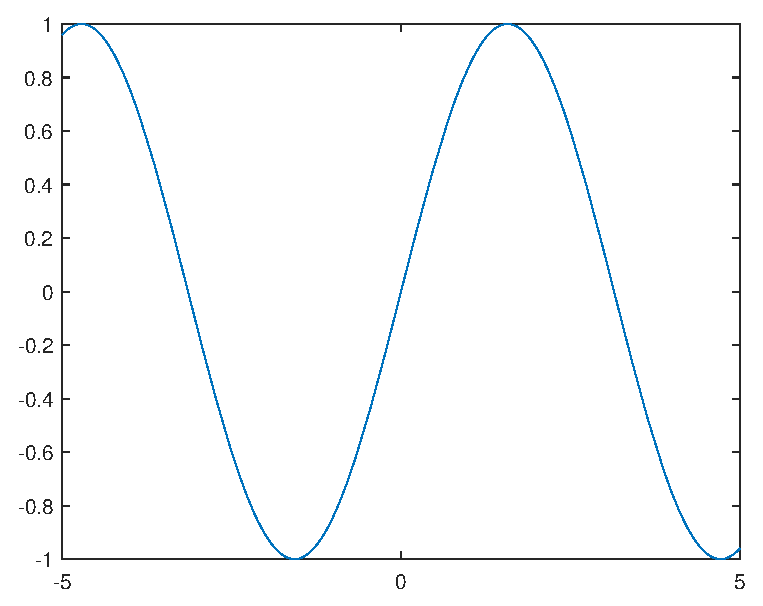
\includegraphics[width=0.6\linewidth]{image1.eps}
\end{figure}
\end{frame}

%------------------------------------------------

\begin{frame}
\frametitle{Two pictures}
\begin{figure}[htb]
\centering
\begin{minipage}{0.48\linewidth}
\centering
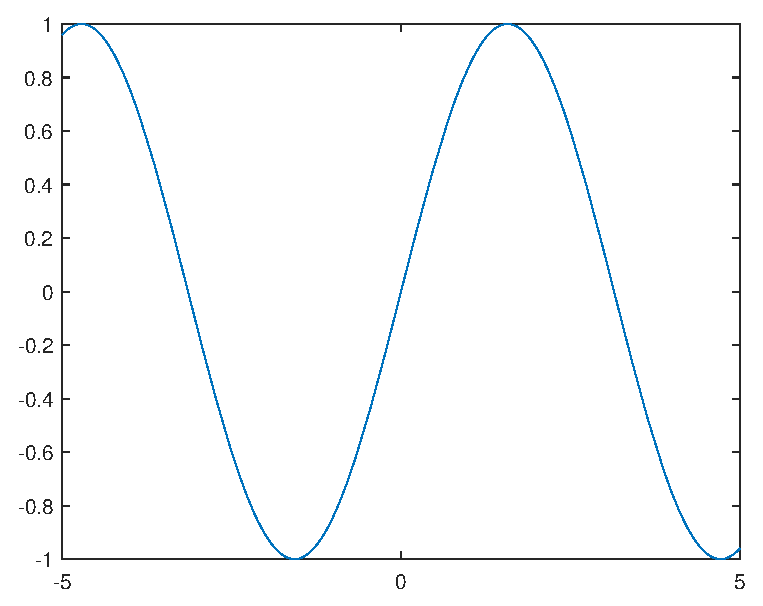
\includegraphics[width=\linewidth]{image1}
\caption{Caption of Figure 1.}
\end{minipage}\hfill
\begin{minipage}{0.48\linewidth}
\centering
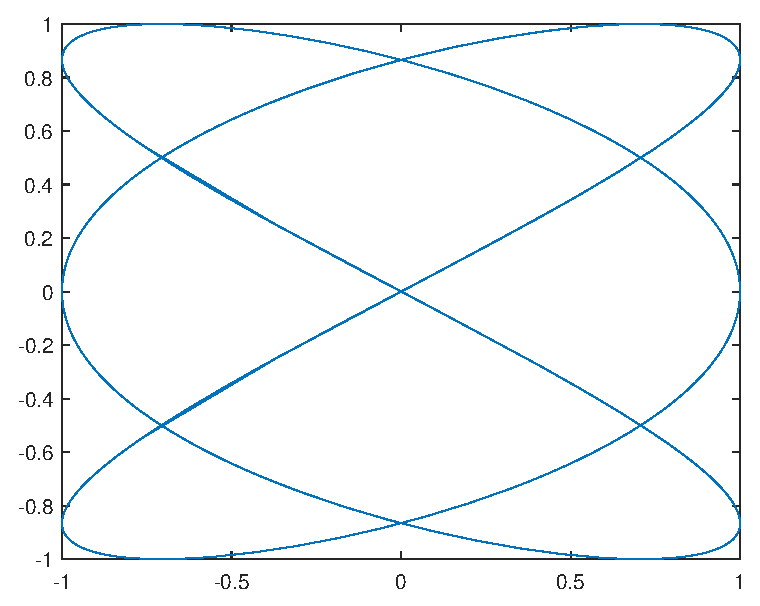
\includegraphics[width=\linewidth]{image2}
\caption{Caption of Figure 2.}
\end{minipage}
\end{figure}
\end{frame}

%------------------------------------------------
\section{Third Section}
%------------------------------------------------

\begin{frame}[fragile] % Need to use the fragile option when verbatim is used in the slide
\frametitle{Citation}
An example of the \verb|\cite| command to cite within the presentation:\\~

This statement requires citation \cite{Smith2012}.
\end{frame}

%------------------------------------------------

\begin{frame}
\frametitle{References}
\footnotesize{
\begin{thebibliography}{99} % Beamer does not support BibTeX so references must be inserted manually as below
\bibitem[Smith, 2012]{Smith2012} John Smith. Title of the publication. \emph{Journal Name}, 12(3):45--678, 2012.
\end{thebibliography}
}
\end{frame}


%------------------------------------------------
%\thispagestyle{empty}
\setbeamertemplate{headline}{}
\setbeamertemplate{footline}{%
  \hfill%
  %\usebeamercolor[fg]{page number in head/foot}%
  \usebeamercolor[gray]{page number in head/foot}%
  \usebeamerfont{page number in head/foot}%
  \insertframenumber \,/\,\inserttotalframenumber
  \kern1em\vskip2pt%
}

%------------------------------------------------
%\setbeamertemplate{background canvas}[vertical shading][bottom=white,top=structure.fg!25]
%\setbeamertemplate{headline}{}
\begin{frame}
\sffamily
\begin{center}
\HUGE{\textcolor[RGB]{165,3,3}{Thank~you!}}
\end{center}
\end{frame}

%------------------------------------------------
%%\setbeamertemplate{background canvas}[vertical shading][bottom=white,top=structure.fg!25]
%\begin{frame}
%\Huge{\centerline{The End}}
%\end{frame}


\end{document}

